\section{Collaboration in Intrusion Detection\label{sec:bg.collab}}

The topic of collaboration in intrusion detection is rather old, with several surveys and reviews available in the literature~\cite{zhou_surveycoordinatedattacks_2010,elshoush_Alertcorrelationcollaborative_2011,vasilomanolakis_TaxonomySurveyCollaborative_2015,meng_CollaborativeSecuritySurvey_2015,folino_Ensemblebasedcollaborative_2016,li_SurveyingTrustBasedCollaborative_2022}, and the oldest references dating back to the early 1990s~\cite{snapp_DIDSdistributedintrusion_1992}.
In this section, we present the different types of collaboration in intrusion detection, and discuss some of the challenges that they face.
A first distinction can be made between their objectives, also they are not mutually exclusive:
\begin{enumerate*}[(i)]
  \item \emph{share results} to correlate alerts and detect attacks at a global scale, or
  \item \emph{share knowledge} to improve the detection capabilities of local systems.
\end{enumerate*}

This distinction also transpires from the scale of the collaboration.
The first case mostly refers to different probes, or sensors, that monitor the same infrastructure, and share their results to correlate alerts and detect attacks at the infrastructure level.
In the second case, which is sometimes referred to as a \gls{cidn}~\cite{li_SurveyingTrustBasedCollaborative_2022}, collaboration usually happens among different organizations or entities that monitor infrastructures.
In this thesis, we will focus on the latter, as it is more relevant to the \gls{fl} context (see \Cref{sec:bg.fl}).


\subsection{The different topologies\label{sec:bg.collab.topo}}

\begin{figure}
  \centering
  \begin{subfigure}{.25\textwidth}
    \centering
    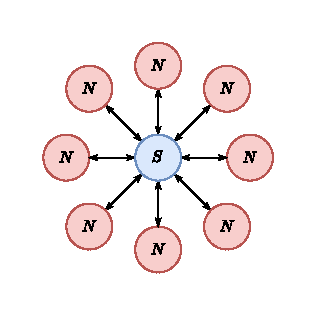
\includegraphics[width=\textwidth]{figures/topo-centralized}
    \caption{Centralized}
    \label{fig:cids.centralized}
  \end{subfigure}%
  \begin{subfigure}{.25\textwidth}
    \centering
    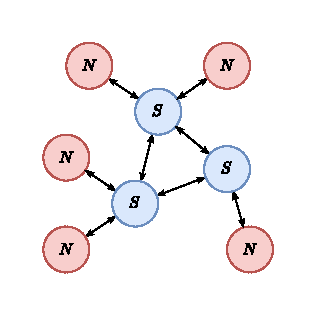
\includegraphics[width=\textwidth]{figures/topo-decentralized}
    \caption{Decentralized}
    \label{fig:cids.decentralized}
  \end{subfigure}%
  \begin{subfigure}{.25\textwidth}
    \centering
    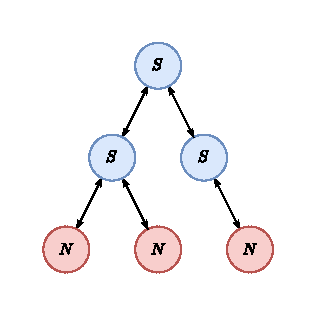
\includegraphics[width=\textwidth]{figures/topo-hierarchical}
    \caption{Hierarchical}
    \label{fig:cids.hierarchical}
  \end{subfigure}%
  \begin{subfigure}{.25\textwidth}
    \centering
    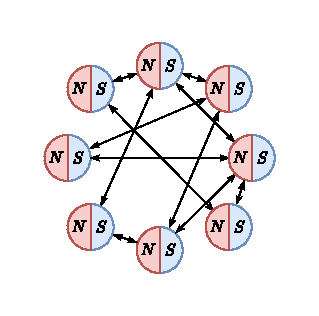
\includegraphics[width=\textwidth]{figures/topo-distributed}
    \caption{Distributed}
    \label{fig:cids.distributed}
  \end{subfigure}
  \caption[
    Different topologies for collaborative intrusion detection systems.
  ]{
    Different topologies for collaborative intrusion detection systems.
    Nodes are in red and marked as $N$, while servers are in blue and marked as $S$.
    Arrows represent connections between entities.
    \label{fig:cids.topoligies}
  } 
\end{figure}

The aforementioned literature identify three main types of topologies for \glspl{cids}: centralized, decentralized, and distributed.
The definitions of these topologies are not always consistent across the literature, especially between the terms \emph{decentralized}, \emph{hierarchical}, and \emph{distributed}.
For instance, \textcite{zhou_surveycoordinatedattacks_2010} consider a decentralized system as a system where each node is autonomous and can make decisions independently, while this definition matches the description of a distributed architecture in the work of \textcite{li_SurveyingTrustBasedCollaborative_2022}.

In this manuscript, we will use the definitions illustrated in \Cref{fig:cids.topoligies}.
It distinguishes two types of roles: \emph{nodes} ($N$) and \emph{servers} ($S$).
A node is a device that captures data, although it can also execute complementary tasks like preprocessing, feature extraction, or traffic analysis.
A server is a device that aggregates the data from the nodes and distributes instructions to them, as well as updates for the local detection algorithm.
The different topologies are defined as follows:
\begin{description}
  \item[Centralized] In a centralized architecture, a single server centralizes knowledge and distributes instructions to the nodes.
  \item[Decentralized] In a decentralized architecture, multiple servers coexist.
    Each server is responsible for a subset of the nodes, and they can share information between them.
  \item[Hierarchical] A hierarchical architecture is decentralized system where the servers are organized in a tree-like structure.
    Each server is responsible for a subset of the nodes, and they can forward information to their parent.
    Likewise, parents can distribute instructions and updates to their children so that they are disseminated throughout the hierarchy.
  \item[Distributed] In a distributed architecture, each node is autonomous and can make decisions independently.
    Both roles of nodes and servers coexist in the same entity.
    There are no servers anymore, and the node share information over a peer-to-peer network.
\end{description}

\Cref{fig:cids.topoligies} illustrates these topologies.
In the centralized architecture (\Cref{fig:cids.centralized}), all nodes are connected to a single server.
\Cref{fig:cids.decentralized} shows a standard example of a decentralized architecture.
\Cref{fig:cids.hierarchical,fig:cids.distributed} illustrate the specific cases of decentralized architectures: hierarchical and distributed, respectively.
The arrows between the different entities represent information exchange, although the nature of these exchanges can vary depending on the direction.
An arrow displayed as $N \rightarrow S$ can represent collected data, generated alerts, or requests for updates.
An arrow displayed as $S \rightarrow N$ can represent instructions or updates for the local detection algorithm or database.

\subsection{Challenges in Collaborative Intrusion Detection\label{sec:bg.collab.challenges}}

Collaborative intrusion detection faces challenges, including the \gls{spof} in a centralized architecture.
If the analysis is performed remotely, like in a \gls{soc} monitoring its consumers' infrastructures, a failure on the central server would hinder detection.
Fortunately, in knowledge-sharing scenarios, detection is (at least partially) performed locally, reducing the impact of a centralized failure.
Nonetheless, collaboration still relies on the availability of the central server.

\begin{challenge}
  \Glspl{cids} typically rely on a central server for coordination and updates, which represent a \acrfull{spof}.
  \label{chall:spof}
\end{challenge}

Another challenge in collaborative intrusion detection is the latency induced by propagating information over the network, especially under load.
The ENISA, the European Union Agency for Cybersecurity, defines the actionability of \gls{ti} as the fulfillment of five criteria: relevance, digestibility, accuracy, completeness, and timeliness~\cite{ENISA2014}.
It is the supporting architecture that provides the latter.
Because low-latency is crucial for actionable alerts locally, centrally analyzing the data increases the time between the event and its detection.

\begin{challenge}
  Centralized detection increases latency, which makes the shared knowledge less actionable.
  \label{chall:actionability}
\end{challenge}

Further, sharing data can represent a privacy risk for a company, as the data relevant for intrusion detection is likely to contain sensitive information~\cite{zhou_surveycoordinatedattacks_2010}.
Exposed information might reveal relevant insights to a competitor or an attacker.


\begin{challenge}
  \Glspl{cids} can expose sensitive information about the internals of a company.
  \label{chall:privacy}
\end{challenge}

A lot of other factors can impede collaboration.
For instance, stakeholders are often reluctant to share their information, fearing confidentiality and privacy issues (see \Cref{chall:privacy}), but most importantly the reputation loss that could result from a breach~\cite{pala_InformationSharingCybersecurity_2019}.
Cultural and language barriers can negatively affect the accuracy of the shared information, even though international collaboration is push by regulation, such as the NIS directives in Europe \cite{NIS_directive,NIS2}.
Finally, the balance between anonymity and trust must be taken into consideration to protect the participants without sacrificing the quality of the information~\cite{murdoch_AnonymityvsTrust_2015}.


\subsection{\Gls{cids} with \acrlong{ml}\label{sec:bg.collab.ml}}

Before the advent of \gls{fl}, the literature on \glspl{cids} leveraging \gls{ml}, or more generally data-mining techniques, was scarce~\cite{folino_Ensemblebasedcollaborative_2016}.
Existing solutions were mostly based sharing alerts for correlation or rules for misuse detection, or rely on a central server to perform learning tasks.
Nonetheless, a few works leveraged distributed learning techniques that remind of \gls{fl}, notably with the constraint of not being able to share data between the nodes.
For instance, \textcite{folino_ensemblebasedevolutionaryframework_2010} proposed a framework allowing distributed \gls{ids} nodes to train and exchange classifiers, before aggregating to build ensemble models.
However, most of the aforementioned reviews still identify data-mining and \gls{ml} techniques as a promising direction for \glspl{cids}.
